\documentclass[tikz]{standalone}

\usepackage[T1]{fontenc}
\usepackage[english]{babel}

\usepackage{standalone}

\usepackage{tikz}
\usetikzlibrary{calc}

\begin{document}
    \begin{tikzpicture}
        \node (3d) at (0,0) {
            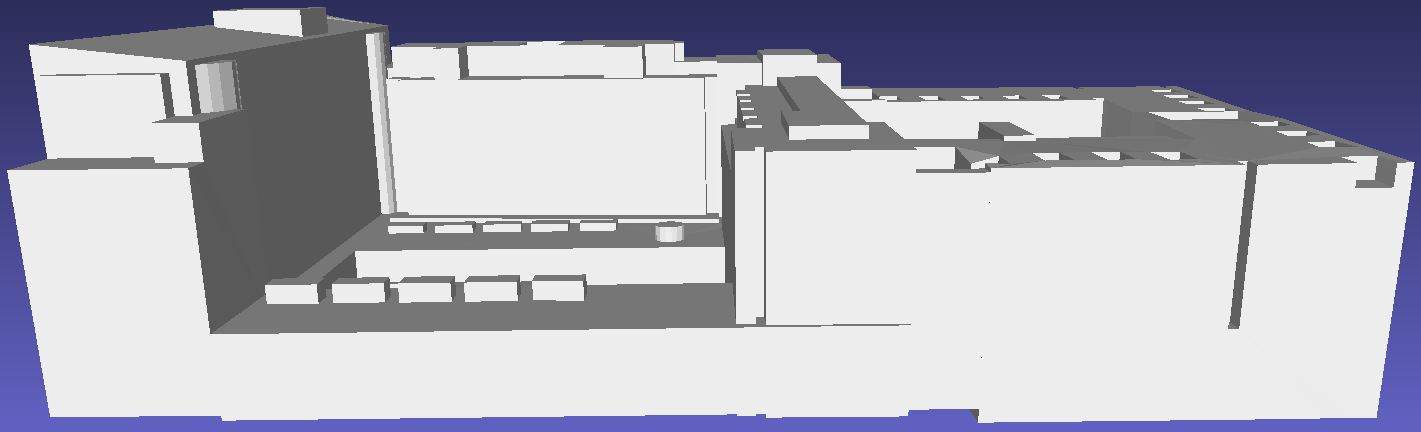
\includegraphics[height=4cm]{images/difference_mesh_model/ground_truth}
        };
        \path (3d) + (4.4, 1.6) node[orange] (facet) {Facet $\equiv$ architectural feature};
        \path (3d) + (.9, .9) node (facet_point) {};
        \path ($(facet.west) ! .8 ! (facet_point)$) node (halfway_facet_point) {};
        \path[draw, ->, orange] (facet.west) -- (halfway_facet_point |- facet.west) -- (facet_point);
    \end{tikzpicture}
\end{document}
